

\section{Forced Choice User Experiment}

\subsection{Recruitment and Participation}

Novice participants were recruited via flyer (figure~\ref{fig:flyer}). An anonymized listing of all participants including demographic information is shown in table~\ref{tab:participants}.

\begin{figure}[t]
\centering

\includegraphics[width=\linewidth]{gfx/flyer_anon.pdf}
\caption{Participants were recruited with this flyer.}
\label{fig:flyer}
\end{figure}

\begin{figure}[t]
\centering
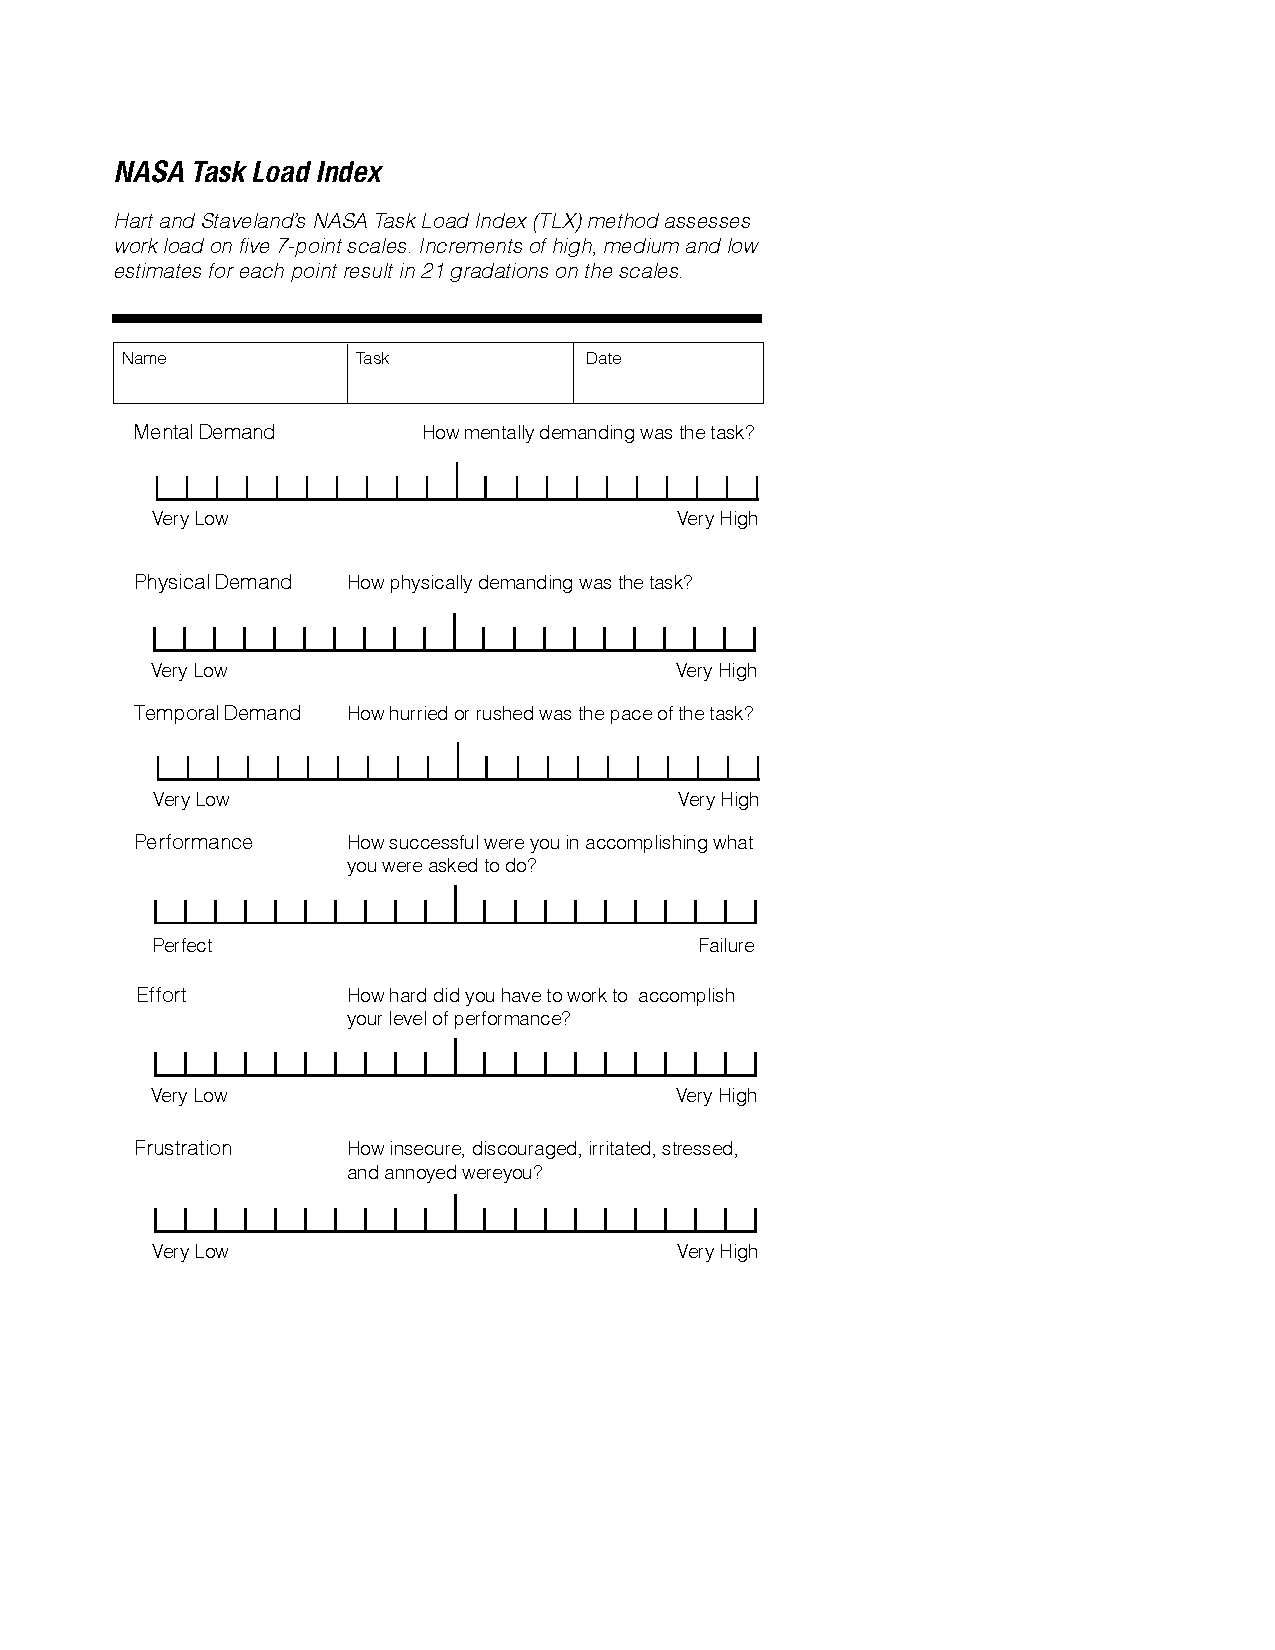
\includegraphics[width=\linewidth]{gfx/NASA_TXL.pdf}
\caption{The NASA-TLX workload index to record subjective responses.}
\label{fig:nasatxl}
\end{figure}


\begin{table}[t]
\caption{The novice participants ($N=20$) of the forced choice user experiment. The table shows sex (20 female), age ($M=30$) and the randomly assigned classifier (focused proofreading as FP, guided proofreading as GP).}%While the training of our classifier is more expensive, testing accuracy is superior. }

\small{
\begin{tabular}{@{}l|c|c|c@{}}
	\toprule
     \textbf{ID} & \textbf{Sex} &  \textbf{Age} & \textbf{Classifier}  \\ \midrule	
S38 &		F & 20 & FP \\
S57&		F & 30 & FP \\ 
S32&		M & 38 & FP \\
S34&		F & 21 & FP \\
S21&		F & 65 & FP \\
S9 &	M & 33 & FP \\
S45 &		M & 28 & FP \\
S31&		M & 27 & FP \\
S24&		F & 21 & FP \\
S6	&	F & 38 & FP \\
S28	&	M&	32& GP \\
S36	&	F&	19& GP \\
S35	&	M&	26& GP \\
S25	&	M&	26& GP \\
S54	&	F&	30& GP \\
S53	&	M&	29& GP \\
S52	&	M	&27& GP \\
S51&		M&	31& GP \\
S200	 &	F	&37& GP \\
S3	 &F&	30 & GP



\end{tabular}
\hspace{2mm}
}
\label{tab:participants}
\end{table}

\subsection{Example Classifications}

During the user study, participants were asked to accept or reject potential errors and their corrections --- some more difficult than others. Figure~\ref{fig:patches} shows a selection of potential errors and their corrections.

\begin{figure}[t]
\centering
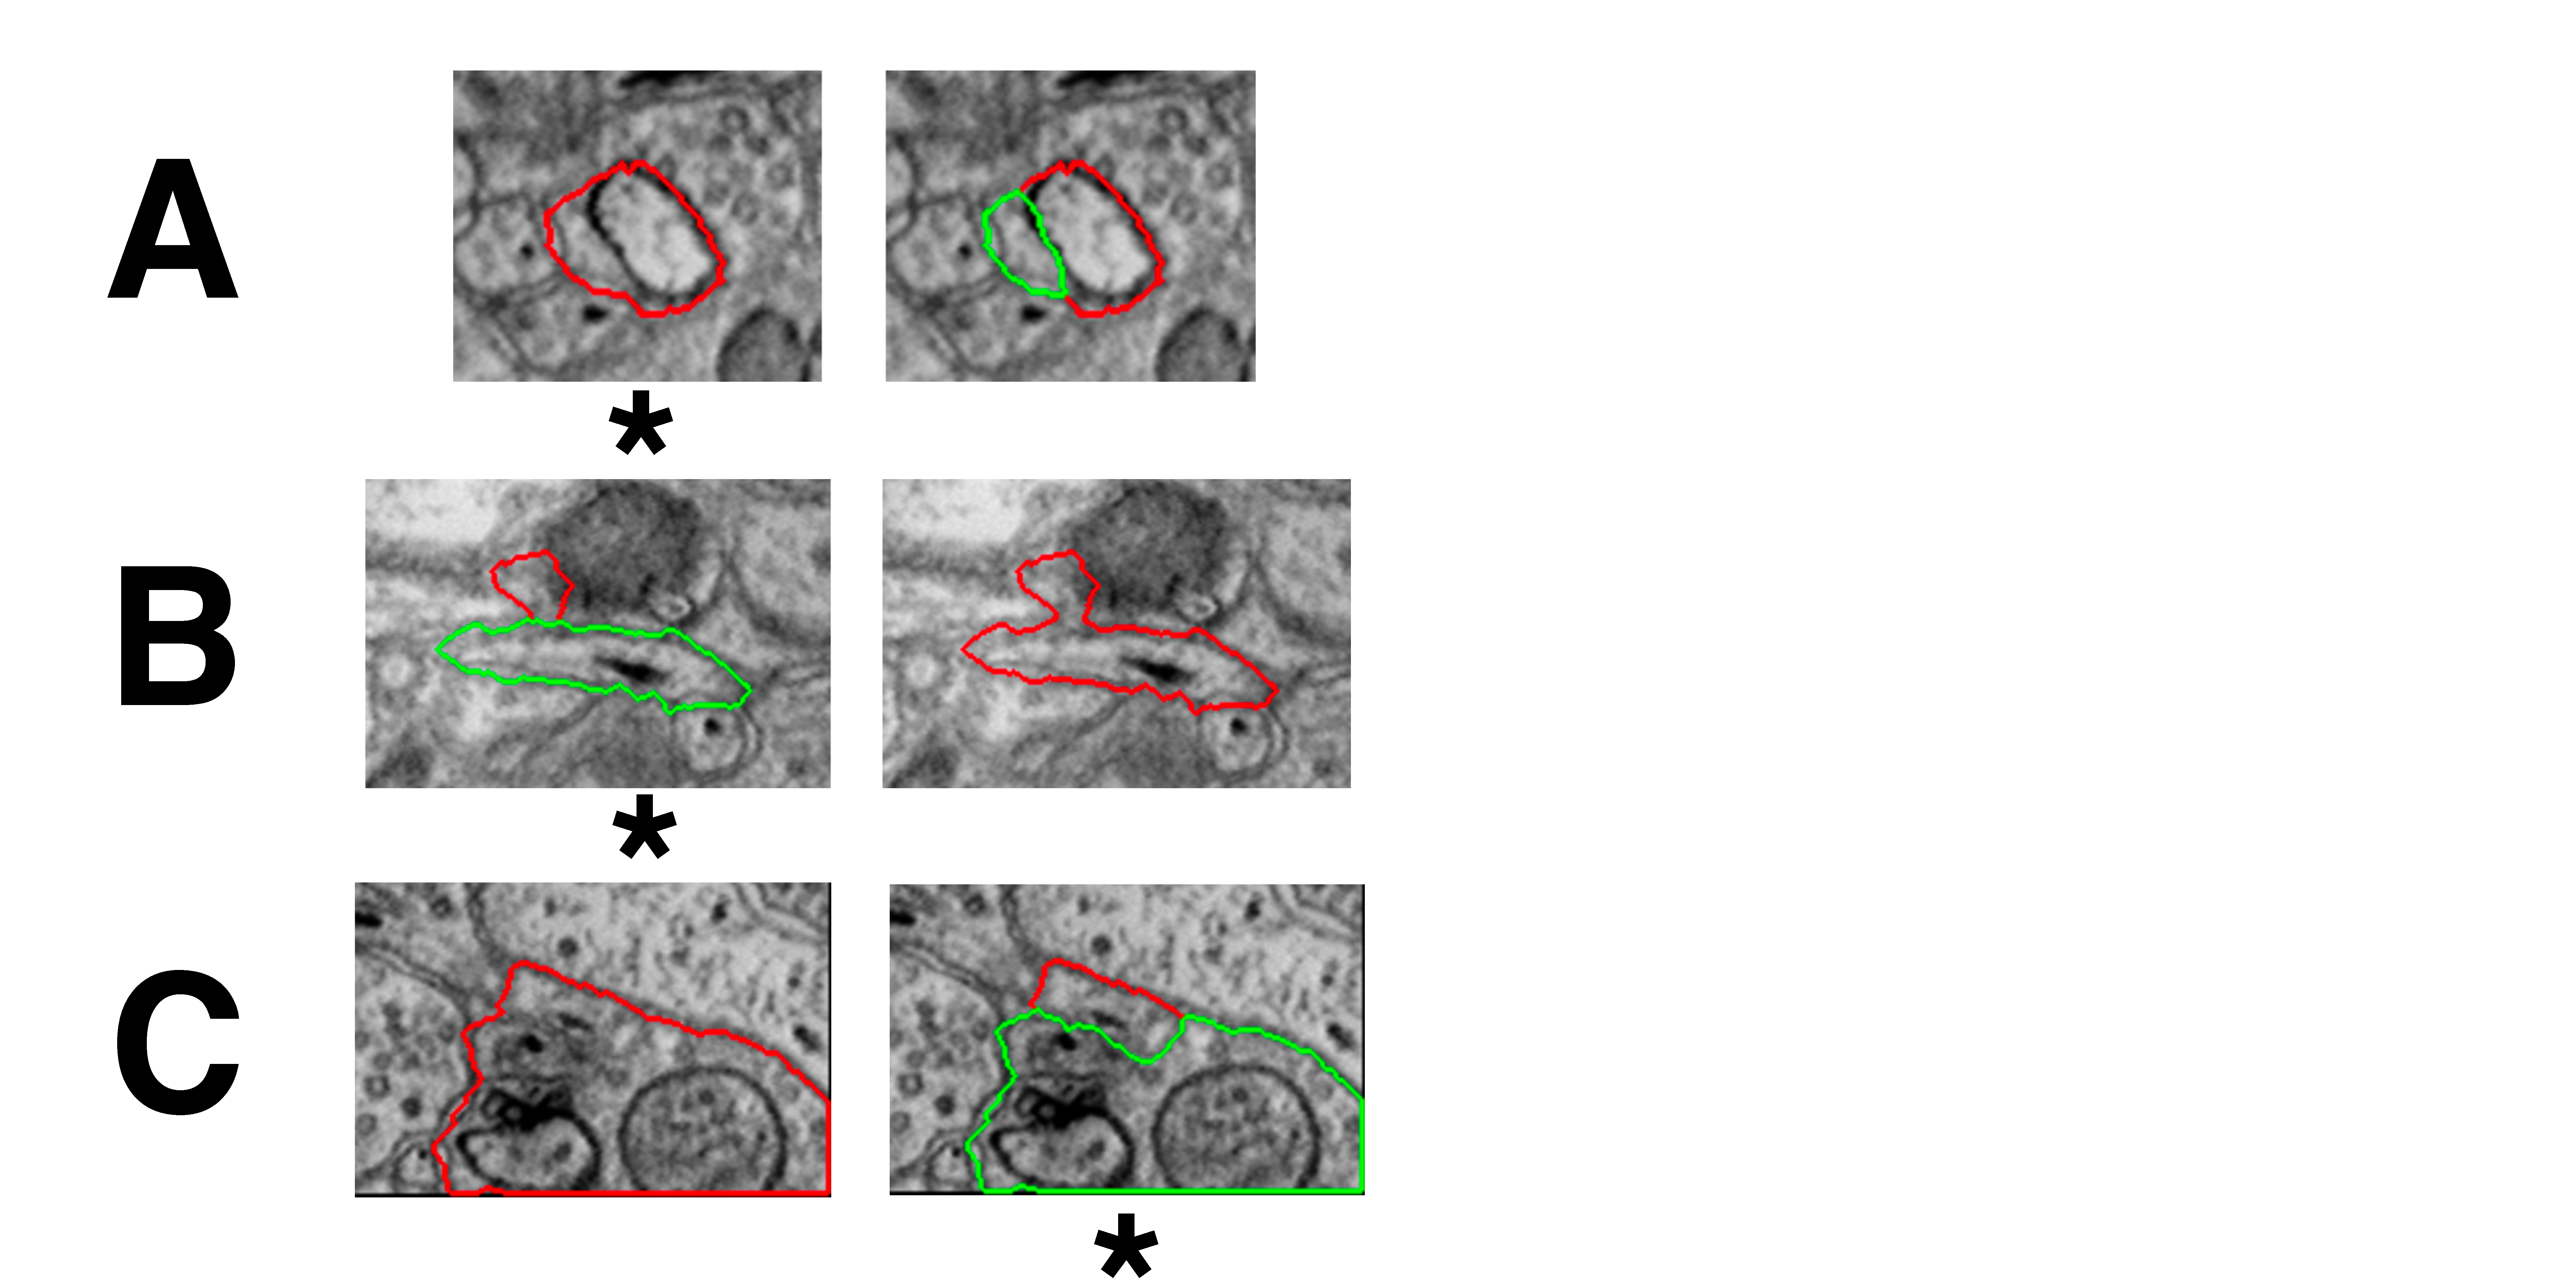
\includegraphics[width=\linewidth]{gfx/patches.pdf}
\caption{A selection of suggested errors and potential corrections during the forced choice user experiment. The star (*) indicates which choice reduces VI. While all participants were able to correctly choose for patch A, only few were able to correctly choose for patch B and C.}
\label{fig:patches}
\end{figure}

\subsection{Subjective Responses}

After the experiment, we acquired subjective responses using the NASA-TLX task load index (Figure~\ref{fig:nasatxl}). We performed ANOVA to test for statistical significance~\cite{shaffer1995}. Mental, physical, and temporal demands were reported slightly higher for participants using focused proofreading but the analysis did not yield any significance.

\begin{itemize}
\item \textbf{Mental Demand.} Participants using focused proofreading stated a higher mental demand $M=11.5$ ($SD=2.098$) than with guided proofreading $M=8.1$ ($SD=2.003$). This was not statistically significant ($F_{1,18}=3.2574, p=0.3695$).
\item \textbf{Physical Demand.} While naturally physical demand was rated low, participants using focused proofreading stated it slightly higher $M=5.4$ ($SD=2.26$) than with guided proofreading $M=2.9$ ($SD=1.76$). This was not statistically significant ($F_{1,18}=1.7507, p=0.5454$).
\item \textbf{Temporal Demand.} For temporal demand, participants using focused proofreading $M=8.4$ ($SD=1.95$) reported almost equal to guided proofreading $M=8.3$ ($SD=1.99$). This was not statistically significant ($F_{1,18}=0.0033, p=0.9987$).
\item \textbf{Performance.} Here, participants were asked to rate their own performance. All participants rated their performance as pretty well (the lower, the better). For focused proofreading $M=6.8$ ($SD=1.97$) and for guided proofreading $M=7.8$ ($SD=2.04$). This was not statistically significant ($F_{1,18}=0.3091, p=0.8878$).
\item \textbf{Effort.} Participants using focused proofreading stated higher effort $M=13.0$ ($SD=2.336$) than with guided proofreading $M=10.6$ ($SD=2.127$). This was not statistically significant ($F_{1,18}=1.1459, p=0.6599$).
\item \textbf{Frustration.} Participants overall reported low frustration. Reported were $M=5.0$ ($SD=1.90$) using focused proofreading and $M=5.9$ ($SD=185$) using guided proofreading. This was not statistically significant ($F_{1,18}=0.3271, p=0.8818$).
\end{itemize}